%   % !TEX root = ../../VIII,3_Rahmen-TeX_8-1.tex
%
%
%   Band VIII, 3 N.~??A20/Y.7
%   Signatur/Tex-Datei: LH_35_09_16_002-003
%   RK-Nr. 41159
%   Überschrift: Extensiones elasticorum sunt viribus tendentibus proportionales
%   Datierung: [März/April 1683 bis erste Hälfte 1684]
%   WZ: 803007 = RK-WZ: 288 (Wz auf Bl. 3; Gegnmarke auf Bl. 2)
%.  SZ: (keins)
%.  Bilddateien (PDF): LH_35_09_16_002-003_d1; LH_35_09_16_002-003_d2; LH_35_09_16_002-003_d3; LH_35_09_16_002-003_d4; LH_35_09_16_002-003_d5; LH_35_09_16_002-003_d6a; LH_35_09_16_002-003_d6b; LH_35_09_16_002-003_d7a; LH_35_09_16_002-003_d7b; LH_35_09_16_002-003_d7c; LH_35_09_16_002-003_d7d (insgesamt: elf)
%
%
\selectlanguage{ngerman}%
\frenchspacing%
%
\begin{ledgroupsized}[r]{120mm}%
\footnotesize%
\pstart%
\noindent%
\textbf{Überlieferung:}%
\pend%
\end{ledgroupsized}%
\begin{ledgroupsized}[r]{114mm}%
\footnotesize%
\pstart%
\parindent -6mm%
\makebox[6mm][l]{\textit{L}}%
Konzept: LH~XXXV~9,~16 Bl.~2\textendash3.
Ein Bogen~2\textsuperscript{o};
ein Wasserzeichen auf Bl.~3 mit Gegenmarke auf Bl.~2:
Papier aus dem Harz.
Zwei stark bearbeitete Seiten auf Bl.~2~v\textsuperscript{o}\! und Bl.~3~r\textsuperscript{o};
Bl.~3~v\textsuperscript{o} ist leer;
Bl.~2~r\textsuperscript{o} und die ersten zwölf Zeilen auf Bl.~2~v\textsuperscript{o} überliefern das Konzept N.~14\textsubscript{6},~\textit{L\textsuperscript{1}},
das von N.~14\textsubscript{7} ursprünglich fortgesetzt wurde.
Die Nummerierung der Diagramme \lbrack\textit{Fig.~1}\rbrack\ bis \lbrack\textit{Fig.~6a}\rbrack\ in N.~14\textsubscript{7} zählte ursprünglich drei in N.~14\textsubscript{6},~\textit{L\textsuperscript{1}} überlieferte Diagramme mit % , nämlich \lbrack\textit{Fig.~1a}\rbrack, \lbrack\textit{Fig.~2a}\rbrack\ und \lbrack\textit{Fig.~5a}\rbrack\ 
(siehe zu N.~14\textsubscript{6}, \textit{L\textsuperscript{1}}, S.~\refpassage{dnr_AE_1684_319-325_Ueberlieferung_csjhfj-1}{dnr_AE_1684_319-325_Ueberlieferung_csjhfj-3}).
Am Kopf von Bl.~2~r\textsuperscript{o}\! Vermerk von Leibnizens Hand:
\textit{Demonstratio quod extensiones Elasticorum sint viribus tendentibus proportionales} \lbrack/\rbrack\ \textit{Verte}
\pend%
\end{ledgroupsized}%
%
%
%
\selectlanguage{latin}%
\frenchspacing%
%
%
\count\Bfootins=1000
\count\Afootins=1100
\count\Cfootins=1100
%
%
% \newpage%
\vspace{8mm}%
\pstart%
\normalsize%
\noindent%
%
\lbrack2~v\textsuperscript{o}\rbrack%%%% Blatt 2v
%
\edtext{}{%
{\xxref{LH_35_09_16_002v_Ueberschrift-1}{LH_35_09_16_002v_Ueberschrift-2}}%
{\lemma{\textso{Demonstratio} \lbrack...\rbrack\ \textso{commeantis}\,}\Cfootnote{%
Die Überschrift wurde als neuer Anfang von N.~14\textsubscript{7} am Rand von Bl.~2~v\textsuperscript{o} ergänzt, nachdem das Teilkonzept N.~14\textsubscript{6},~\textit{L\textsuperscript{1}} auf Bl.~2~r\textsuperscript{o} und in der ersten Zeilen von Bl.~2~v\textsuperscript{o} gestrichen worden war.%
% ersetzt den gestrichenen Textabschnitt \textit{Scientia Mechanica} \lbrack...\rbrack\ \textit{est Galilaeo}
% (S.~\refpassage{LH_35_10_16_002_Anfang-1}{LH_35_10_16_002_Anfang-2}).
}}}%
%
\textso{ Demonstratio}\edlabel{LH_35_09_16_002v_Ueberschrift-1}%
\protect\index{Sachverzeichnis}{demonstratio}\textso{ nova,
quod chordarum,}\protect\index{Sachverzeichnis}{chorda elastica}%
\textso{ aliorumque corporum }%
\edtext{\textso{solido\-rum}\protect\index{Sachverzeichnis}{corpus solidum}}{%
\lemma{\textso{solidorum}}\Bfootnote{\textit{erg.~L}}}%
%
\textso{ Elasticorum}\protect\index{Sachverzeichnis}{corpus elasticum}%
\textso{ extensiones}\protect\index{Sachverzeichnis}{extensio elastici}%
\textso{ sint viribus tendentibus}\protect\index{Sachverzeichnis}{vis tendens}%
\textso{ proportionales,}\protect\index{Sachverzeichnis}{extensio proportionalis}%
\textso{ ex hypothesi fluidi }%
\protect\index{Sachverzeichnis}{hypothesis fluidi elastici}\protect\index{Sachverzeichnis}{fluidum elasticum}%
\edtext{\textso{Elastici in eorum poris existentis,}}{%
\lemma{\textso{Elastici}}\Bfootnote{%
\textit{(1)}~\textso{permeantis}
\textit{(2)}~\textso{in eorum poris existentis,}%
~\textit{L}}}\protect\index{Sachverzeichnis}{porus}%
%
\textso{ non tamen satis libere per eos commeantis}\edlabel{LH_35_09_16_002v_Ueberschrift-2}
\pend%
\vspace*{1.0em}%
%
\pstart%
\noindent%
Sit\edlabel{LH_35_09_16_002_Beweis-1} in\protect\index{Sachverzeichnis}{figura}
\edtext{fig.~1}{%
{\lemma{fig.}\Bfootnote{%
\textit{(1)}~4
\textit{(2)}~1%
~\textit{L}}}%
{\lemma{fig.~1}\Cfootnote{%
Das Diagramm \lbrack\textit{Fig.~1}\rbrack\ auf 
S.~\pageref{LH_35_09_16_002v_Fig.1}.}}}
%
chorda \textit{AB} nullo modo tensa,\protect\index{Sachverzeichnis}{chorda tensa}
sed in statu naturali constituta,\protect\index{Sachverzeichnis}{status naturalis}
quae appenso pondere\protect\index{Sachverzeichnis}{pondus appensum}
\edtext{\lbrack\textit{E}\rbrack}{%
\lemma{\textit{E}}\Bfootnote{\textit{erg. Hrsg.}}}
%
extendatur a \textit{B} usque ad \textit{C},
appenso autem pondere\protect\index{Sachverzeichnis}{pondus appensum}
\edtext{\lbrack\textit{F}\rbrack}{\lemma{\textit{D}}\Bfootnote{\textit{L~ändert Hrsg.}}}
%
extendatur a \textit{B} usque
\edtext{ad \textit{D},\textso{ ajo pondera tendentia fore}%
\protect\index{Sachverzeichnis}{pondus tendens}}{%
\lemma{ad}\Bfootnote{%
\hspace{-0,5mm}\textit{D},
\textit{(1)}~\textso{erunt}
\textit{(2)}~\textso{ajo pondera tendentia fore}%
~\textit{L}}}%
%
\textso{ extensionibus proportionalia,}\protect\index{Sachverzeichnis}{extensio chordae}
seu \textit{E} ad \textit{F} ut \textit{BC} ad \textit{BD}.
\edtext{Quae
\edtext{quidem propositio\protect\index{Sachverzeichnis}{propositio}}{%
\lemma{quidem}\Bfootnote{%
\textit{(1)}~Hypothesis
\textit{(2)}~propositio%
~\textit{L}}}
%
demonstrari potest adhibito aere\protect\index{Sachverzeichnis}{aer ordinarius}
vel alio fluido Elastico\protect\index{Sachverzeichnis}{fluidum elasticum}}{%
\lemma{Quae \lbrack...\rbrack\ Elastico}\Cfootnote{%
Siehe hierzu die Aufzeichnung LH~XXXVII~3 Bl.~125\textendash127
(sie soll in \textit{LSB} VIII veröffentlicht werden).}}
%
\edtext{quod tanquam homogeneum\protect\index{Sachverzeichnis}{fluidum homogeneum} concipitur,}{%
\lemma{quod}\Bfootnote{%
\hspace{-0,5mm}tanquam homogeneum concipitur
\textit{erg.~L}}}
%
si quidem chordarum\protect\index{Sachverzeichnis}{elastrum chordae}
vel aliorum corporum crassiorum\protect\index{Sachverzeichnis}{elastrum corporis}
Elastrum ab eo
\edtext{oriri ponatur.}{%
\lemma{oriri}\Bfootnote{%
\textit{(1)}~concipiatur.
\textit{(2)}~ponatur.%
~\textit{L}}}
%
Sit\edlabel{LH_35_09_16_002v_asseruimus-1} enim Tubus\protect\index{Sachverzeichnis}{tubus} \textit{AB}
apertus in \textit{A} clausus \makebox[1.0\textwidth][s]{in \textit{B},\textso{ }%
\edtext{\textso{figura}\textso{~2,}\protect\index{Sachverzeichnis}{figura}}{%
{\lemma{\textso{figura}}\Bfootnote{%
\textit{(1)}~\textso{5,}
\textit{(2)}~\textso{2,}%
~\textit{L}}}
{\lemma{\textso{figura~2}\,}%
\Cfootnote{Das Diagramm \lbrack\textit{Fig.~2}\rbrack\ auf 
S.~\pageref{LH_35_09_16_002v_Fig.2}.}}}%
\textso{ }pars \textit{BC} plena aere\protect\index{Sachverzeichnis}{aer ordinarius}
\edtext{ordinario.
Embolus\protect\index{Sachverzeichnis}{embolus}}{%
\lemma{ordinario}\Bfootnote{%
\hspace{-0,5mm}\textbar~seu in statu naturali \textit{gestr.}~%
\textbar~. Embolus%
~\textit{L}}}
%
\textit{LM} extrahendo promoveatur}
\pend
\newpage
\pstart
\noindent a \textit{C} usque
ad \textit{E}.
Dico vim necessariam extractioni priori%
\protect\index{Sachverzeichnis}{vis necessaria extractioni}\protect\index{Sachverzeichnis}{extractio}
fore ad vim necessariam extractioni posteriori%
\protect\index{Sachverzeichnis}{vis necessaria extractioni}\protect\index{Sachverzeichnis}{extractio}
ut
\textit{CD}
\edlabel{KZeitz89}\edtext{}{{\xxref{KZeitz89}{KZeitz90}}%
{%
\lemma{ad}\Bfootnote{%
\hspace{-0,5mm}\textit{CE}.
\textit{(1)}~Nam aer externus qui Elastro aut pondere suo, aut potius utroque Embolum introrsum in tubum pellere conatur, impeditur vi Elastica aeris inclusi.%
\protect\index{Sachverzeichnis}{elastrum aeris}\protect\index{Sachverzeichnis}{pondus aeris}
Constat autem (etiam experimentis)\protect\index{Sachverzeichnis}{experimentum}
\textit{(a)}~vim Elasticam aeris\protect\index{Sachverzeichnis}{vis aeris}
\textit{(b)}~eam
\textit{(c)}~vim elasticam\protect\index{Sachverzeichnis}{vis elastica}
\textit{(d)}~vim aeris inclusi diminui proportione aucti spatii quod ipsi conceditur ultra spatium ordinarium;
quicquid autem decedit de vi Elastica aeris inclusi dandum est potentiae extrahenti,\protect\index{Sachverzeichnis}{potentia extrahens}
quae scilicet inter extrahendum sustinere debet embolum contra vim aeris externi.
Scio quidem quae de pondere et Elastro aeris a
Torricellio,\protect\index{Namensregister}{\textso{Torricelli} (Torricellius), Evangelista 1608\textendash1647}
Pascalio,\protect\index{Namensregister}{\textso{Pascal} (Pascalius), Blaise 1623\textendash1662}
Gerickio\protect\index{Namensregister}{\textso{Guericke} (Gerickius, Gerick.), Otto von 1602\textendash1686}
et Boylio\protect\index{Namensregister}{\textso{Boyle} (Boylius, Boyl), Robert 1627\textendash1691}
asserta sunt quibusdam nondum adhuc probari, sed a me tamen habentur pro demonstratis, et brevitatis causa nunc supponuntur
\textbar~praesertim cum revera eodem res redeat sive
\textit{(1)}~dicas
\textit{(2)}~Elastrum statuas quo se aer dilatare conetur,\protect\index{Sachverzeichnis}{dilatatio aeris}
sive funiculum quod se conetur contrahere,\protect\index{Sachverzeichnis}{funiculum}
cum revera neutrum conatum per se, sed potius ab Aetheris motu habeat;\protect\index{Sachverzeichnis}{motus aetheris}
nec referat an dicas aeris inclusi funiculum suspensum sustinere Mercurium,\protect\index{Sachverzeichnis}{mercurius}
dum aeris externi
\textit{(a)}~cylinder\protect\index{Sachverzeichnis}{cylinder aeris}
\textit{(b)}~pondus sustinetur ab aeris externi superioris funicolo;
an potius dicas aeris externi pondus sustinere Mercurium \textit{erg.}~\textbar~.
\textit{(2)}~Nam aer \lbrack...\rbrack\ occupat spatium
\textbar~proportione \textit{erg.}~%
\textbar\ majus externo, \lbrack...\rbrack\ sint effectis % cumque causae
\textit{(a)}~uniformis
\textit{(b)}~homogeneis proportionales,
\textit{(aa)}~causaque
\textit{(bb)}~effectusque sit difformitas
\textbar~seu differentia consistentiae inter aerem internum et externum \textit{erg. u. gestr.}~%
\textbar\ ab aucto \lbrack...\rbrack\ proportionales. Motum % spatio aeris inclusi, utique vires spatium augentes seu embolum extrahentes, erunt extractionibus
\textit{(aaa)}~autem
\textit{(bbb)}~enim aetheris \lbrack...\rbrack\ sumtis constat.%
% difformitate illa turbari; atque inde vim elasticam seu conatum uniformitatis oriri alias dictum est. Idem experimentis hydrargyro in aere
~\textit{L}}}}%
ad \textit{CE}.
% % % %  ZWEI MARGINALIEN: Anfang des Bezugsbereichs
\edtext{}{{\xxref{KZeitz89}{KZeitz90}}%
{%
% Hier ist der Körper der zweifachen Marginalie = Afootnote
\lemma{\textit{Am Rand:}}\Afootnote{%
Demonstrandum hoc accuratius.
\textit{Nachträglich hinzugefügt:}
Aer ordinarius\protect\index{Sachverzeichnis}{aer ordinarius}
in \protect\rule[-2mm]{0mm}{7mm}vacuo\protect\index{Sachverzeichnis}{vacuum} positus
sustinebit $\mercury$ = \textit{a}\protect\index{Sachverzeichnis}{mercurius} % //??Mercur//
talis scilicet aer qualis est in \textit{BC},
ut Aer\protect\index{Sachverzeichnis}{aer dilatatus} % //in ??// 
dilatatus in \textit{BD} sustinet $\displaystyle\frac{1}{2}a,$
in \textit{BE} $\displaystyle\frac{1}{3}a$ $\mercury\text{\textsuperscript{ii}}$ etc.
Ergo ad \protect\rule[-2mm]{0mm}{7mm}trahendum \textit{M} in \textit{D} opus est pondere $\displaystyle\frac{1}{2}a,$\protect\index{Sachverzeichnis}{pondus extrahens}
ad trahendum in \textit{E} opus est pondere $\displaystyle\frac{2}{3}a.$
Et generaliter si \textit{EB}~:~\textit{EC} sit \textit{x},
erit vis \protect\rule[-2mm]{0mm}{6mm}aeris inclusi elastica residua: 4~:~\textit{x}.%
\protect\index{Sachverzeichnis}{vis elastica}\protect\index{Sachverzeichnis}{aer inclusus}%
\protect\index{Sachverzeichnis}{vis aeris}\protect\index{Sachverzeichnis}{vis residua}
Pondus autem quo ad \textit{E} usque  \protect\rule[-2mm]{0mm}{7mm}extrahendus embolus,\protect\index{Sachverzeichnis}{embolus}\protect\index{Sachverzeichnis}{pondus extrahens}
erit $\displaystyle\frac{x-1}{x}a.$
Itaque in talibus Elasticis\protect\index{Sachverzeichnis}{elasticum}
non sunt extensiones,\protect\index{Sachverzeichnis}{extensio non proportionalis}
ut vires tendentes.\vspace{-8mm}\protect\index{Sachverzeichnis}{vis tendens}}}}%
Nam\edlabel{LH_35_09_16_002_erstzng-1} aer esternus\protect\index{Sachverzeichnis}{aer externus}
et tubo inclusus sunt in aequilibrio,\protect\index{Sachverzeichnis}{aequilibrium}
seque continent in statu uniformitatis,%
\protect\index{Sachverzeichnis}{status uniformitatis}\protect\index{Sachverzeichnis}{uniformitas}
vis autem Elastica\protect\index{Sachverzeichnis}{vis elastica}
nascitur ex difformitate,\protect\index{Sachverzeichnis}{difformitas}
dum verbi gratia aer internus\protect\index{Sachverzeichnis}{aer internus}
occupat spatium\protect\index{Sachverzeichnis}{spatium aeris}
proportione majus externo,\protect\index{Sachverzeichnis}{aer externus}
cumque causae sint effectis homogeneis proportionales,%
\protect\index{Sachverzeichnis}{causa proportionalis}\protect\index{Sachverzeichnis}{effectus homogeneus}
effectusque sit difformitas\protect\index{Sachverzeichnis}{difformitas effectus}
ab aucto spatio aeris inclusi,\protect\index{Sachverzeichnis}{aer inclusus}
utique vires\protect\index{Sachverzeichnis}{vis extrahens}
spatium augentes\protect\index{Sachverzeichnis}{spatium aeris}
seu embolum\protect\index{Sachverzeichnis}{embolus}
extrahentes,\protect\index{Sachverzeichnis}{vis extrahens}
erunt extractionibus\protect\index{Sachverzeichnis}{extractio} \makebox[1.0\textwidth][s]{proportionales.\edlabel{LH_35_09_16_002v_asseruimus-2}
%
\edlabel{KZeitz91}\edtext{}{{\xxref{KZeitz91}{KZeitz92}}%
{%
\lemma{Motum \lbrack...\rbrack\ est}\Cfootnote{%
Siehe etwa \cite{00256}G.\,W. \textsc{Leibniz}, \textit{Hypothesis physica nova}, Mainz 1671, §~27 (\textit{LSB} VI,~2 N.~40, S.~234f.).}}}%
Motum enim aetheris\protect\index{Sachverzeichnis}{motus aetheris}\protect\index{Sachverzeichnis}{aether}
difformitate\protect\index{Sachverzeichnis}{difformitas} illa turbari;
atque inde vim elasticam\protect\index{Sachverzeichnis}{vis elastica}}
\pend
\newpage
\pstart\noindent
\begin{minipage}[t]{0.5\textwidth}
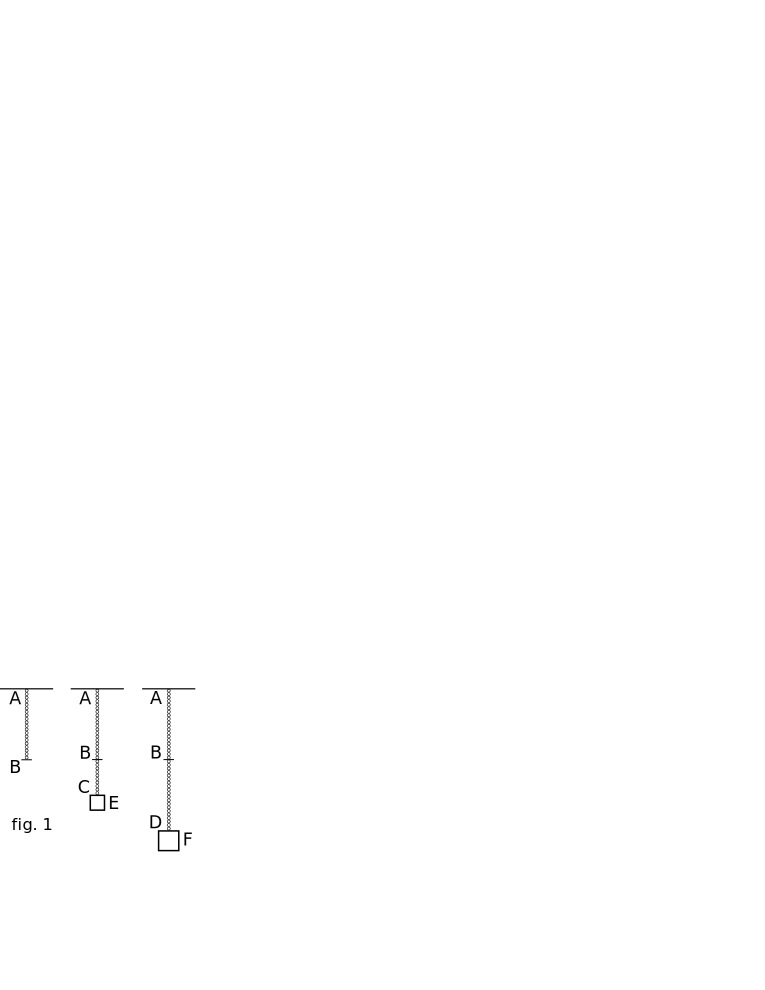
\includegraphics[width=0.66\textwidth]{gesamttex/edit_VIII,3/images/LH_35_09_16_002-003_d1.pdf}
\end{minipage}
\hspace{-2mm}
\begin{minipage}[t]{0.5\textwidth}
\includegraphics[width=0.97\textwidth]{gesamttex/edit_VIII,3/images/LH_35_09_16_002-003_d2.pdf}
\end{minipage}
\\
\\
\hspace*{15mm} [\textit{Fig.~1}] \label{LH_35_09_16_002v_Fig.1}\hspace*{69mm} [\textit{Fig.~2}]\label{LH_35_09_16_002v_Fig.2}%
\pend
  \vspace{2.0em}%
\pstart
\noindent
\edtext{}{\lemma{\hspace{1,1mm}
\lbrack\textit{Fig.~1}\rbrack}\killnumber\Cfootnote{%
Das Diagramm hieß ursprünglich \textit{fig.~4}.}}%
\edtext{}{\lemma{%\hspace{1,6mm}
\lbrack\textit{Fig.~2}\rbrack}\killnumber\Cfootnote{%
Das Diagramm hieß ursprünglich \textit{fig.~5}.}}%
\setline{1}seu conatum uniformitatis\protect\index{Sachverzeichnis}{conatus uniformitatis}
oriri alias dictum est.\edlabel{KZeitz92}
%
\edtext{Idem experimentis hydrargyro in aere sumtis constat.%
\edlabel{LH_35_09_16_002_erstzng-2}\edlabel{LH_35_09_16_002_Beweis-2}}{%
\lemma{Idem \lbrack...\rbrack\ constat}\Cfootnote{%
Wie die Variante \textit{(1)} zum Textabschnitt \textit{Nam aer} \lbrack...\rbrack\ \textit{sumtis constat}
(\refpassage{LH_35_09_16_002_erstzng-1}{LH_35_09_16_002_erstzng-2}) zeigt,
meint Leibniz insbesondere die Experimente von
E.~Torricelli, % \cite{00107}
B.~Pascal, % \cite{00081} + \cite{00234}
O.~von Guericke % \cite{00055}
und R.~Boyle. % \cite{00015}
Siehe \textit{LSB} VIII,~1 N.~39, S.~306.\cite{01069}
In der Variante\,\textit{(1)} erwähnt Leibniz zudem die alternative, auf der \glqq Funiculus-Hypothese\grqq\ beruhende Erklärung,
die auf F.~\textsc{Linus}, \textit{Tractatus de corporum inseparabilitate}, London 1661,\cite{00072} zurückgeht.%
\protect\index{Sachverzeichnis}{funiculum}\protect\index{Namensregister}{\textso{Line} (Linus), Francis 1595-1675}
Siehe \textit{LSB} VIII,~1 N.~40, S.~326.9\textendash18.\cite{01265}}}%
\edlabel{KZeitz90}%%
% % % %  ZWEI MARGINALIEN: Ende
% % % % % %       A C H T U N G   G E T R I X T       ! ! ! ! ! 
% % % % % %
\pend%
%%  \newpage%					Diagramm Fig.~1
%  \vspace*{3.5em}%
%  \centerline{\hspace*{-85mm}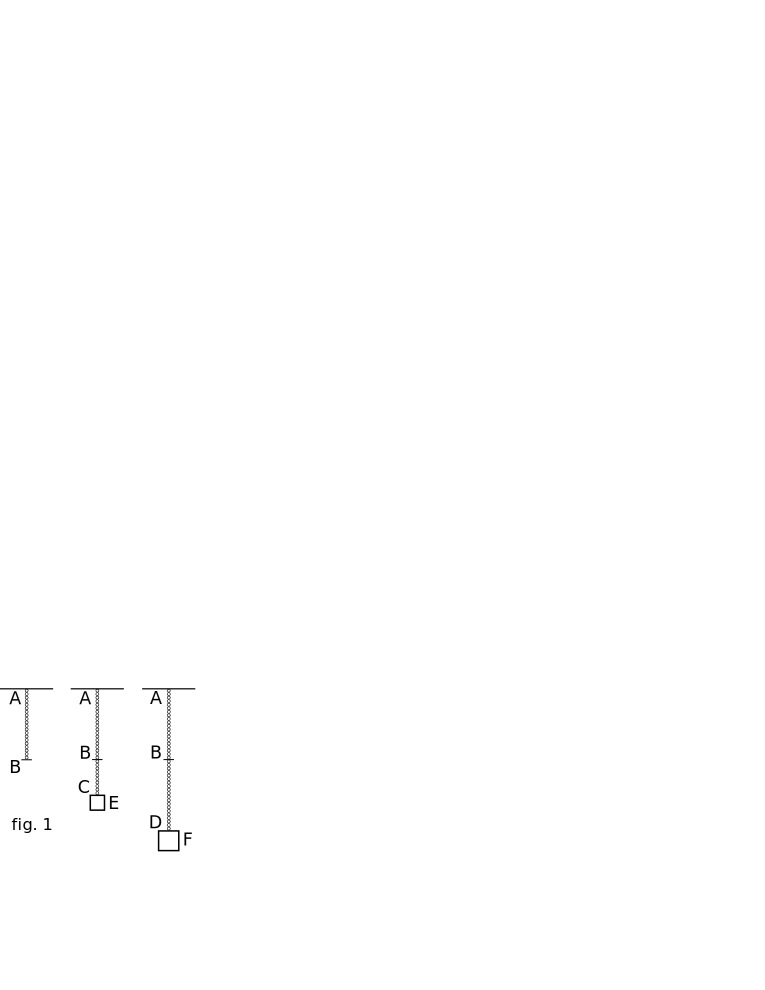
\includegraphics[width=0.32\textwidth]{gesamttex/edit_VIII,3/images/LH_35_09_16_002-003_d1.pdf}}%\\
%  \vspace*{0.0em}
%  \centerline{\hspace*{-85mm}\lbrack\textit{Fig.~1}\rbrack}%
%  \label{LH_35_09_16_002v_Fig.1}%
%%
%%  \newpage%					Diagramm Fig.~2
%  \vspace*{-12.5em}%
%  \centerline{\hspace*{65mm}\includegraphics[width=0.46\textwidth]{gesamttex/edit_VIII,3/images/LH_35_09_16_002-003_d2.pdf}}%\\
%  \vspace*{1.0em}
%  \centerline{\hspace*{65mm}\lbrack\textit{Fig.~2}\rbrack}%
%  \label{LH_35_09_16_002v_Fig.2}%
%
%%  \newpage%					Diagramm Fig.~3
  %\newpage%
%
\count\Bfootins=900
\count\Afootins=1000
\count\Cfootins=1000
\pstart%
Sed 
\edlabel{LH_35_09_16_002v_Festigkeitsmodell_redg-1}
forte dubitabit aliquis % \edtext{}{\lemma{dubitabit aliquis}\Cfootnote{???? Etwa Anspielung ????}} %
quomodo chordarum aliorumque corporum
\edtext{solidorum}{%
\lemma{solidorum}\Bfootnote{\textit{erg.~L}}}
%
tensio\protect\index{Sachverzeichnis}{tensio chordae}\protect\index{Sachverzeichnis}{tensio corporis solidi}\protect\index{Sachverzeichnis}{corpus solidum}
derivari possit ab Elastro alicuius corporis fluidi,%
\protect\index{Sachverzeichnis}{elastrum corporis fluidi}\protect\index{Sachverzeichnis}{corpus fluidum}
\edtext{nam\textso{ primo }}{%
\lemma{nam}\Bfootnote{%
\textit{(1)}~praeterquam quod
\textit{(2)}~\textso{primo}%
~\textit{L}}}%
%
\edtext{Horologia
\edtext{portatilia\protect\index{Sachverzeichnis}{horologium portatile}
laminis chalybeis\protect\index{Sachverzeichnis}{lamina chalybea}}{%
\lemma{portatilia}\Bfootnote{%
\textit{(1)}~Elastris
\textit{(2)}~laminis chalybeis%
~\textit{L}}}
instructa non minus procedunt in aere dilatato\protect\index{Sachverzeichnis}{aer dilatatus}
sive in vacuo Magdeburgico,\protect\index{Sachverzeichnis}{vacuum Magdeburgicum}
quam in aere communi;\protect\index{Sachverzeichnis}{aer communis}}{%
\lemma{Horologia \lbrack...\rbrack\ communi}\Cfootnote{%
Vgl. O.~v. \textsc{Guericke}, \textit{Experimenta nova}, l.~III, cap. 15, Amsterdam 1672, S.~91f.\cite{00055} Zu diesem Versuch \textit{De sono in vacuo} hat Leibniz einen Auszug verfasst: \textit{LSB} VIII,~1 N.~36, S.~256f.\cite{01197}}}%
%
\textso{ }%
\edtext{\textso{secundo}}{%
\lemma{\textso{secundo}}\Bfootnote{\textit{erg.~L}}}%
%
\textso{ }non videtur probabile
tubos\protect\index{Sachverzeichnis}{tubus} atque embolos\protect\index{Sachverzeichnis}{embolus}
\edtext{exacte tubis respondentes,}{%
\lemma{exacte}\Bfootnote{%
\hspace{-0,5mm}tubis respondentes,
\textit{erg.~L}}}
%
ubique in chordis\protect\index{Sachverzeichnis}{chorda elastica}
aut laminis Elasticis\protect\index{Sachverzeichnis}{lamina elastica}
fingere.
Sed sciendum
\edlabel{KZeitz83}\edtext{}{{\xxref{KZeitz83}{KZeitz84}}%
{%
\lemma{est}\Bfootnote{%
\textit{(1)}~ex vacuo Magdeburgico ita di
\textit{(2)}~quoad \textso{primum,} \lbrack...\rbrack\ vacuum dicunt % ex Recipiente quem‚
\textit{(a)}~superesse
\textit{(b)}~exhauriri solummodo aerem crassiorem, superesse%
~\textit{L}}}}%
\makebox[1.0\textwidth][s]{est quoad\textso{ primum,}
ex Recipiente quem vacuum dicunt\protect\index{Sachverzeichnis}{recipiens vacuum}
exhauriri solummodo
aerem}
\pend
\newpage
  \centerline{\includegraphics[width=0.81\textwidth]{gesamttex/edit_VIII,3/images/LH_35_09_16_002-003_d3.pdf}}%\\
  \vspace{0.5em}
  \centerline{\lbrack\textit{Fig.~3}\rbrack}%
  \label{LH_35_09_16_002v_Fig.3}%
%
 \vspace{1.5em}%
\pstart
\noindent\edtext{}{\lemma{\hspace{1,1mm}
\lbrack\textit{Fig.~3}\rbrack}\killnumber\Cfootnote{%
Das Diagramm hieß ursprünglich \textit{fig.~6}.}}%
crassiorem,\protect\index{Sachverzeichnis}{aer crassior}
superesse\edlabel{KZeitz84}
%
vero alium
\edtext{subtiliorem,\protect\index{Sachverzeichnis}{aer subtilior}
qui}{%
\lemma{subtiliorem,}\Bfootnote{\hspace{-0,5mm}% 
\textbar~etiam Elasticum \textit{erg. u. gestr.}~\textbar\ qui%
~\textit{L}}}
%
\edtext{per intervalla corporum majora transire potest,\protect\index{Sachverzeichnis}{intervalla corporum}
licet excludatur}{%
\lemma{per}\Bfootnote{%
\textit{(1)}~poros
\textit{(2)}~intervalla corporum
\textit{(a)}~transire potest, majores
\textit{(b)}~majora transire potest,
\textit{(aa)}~excludatur tamen
\textit{(bb)}~licet excludatur%
~\textit{L}}}
%
a
\edtext{minoribus;
unde ille}{%
\lemma{minoribus;}\Bfootnote{%
\textit{(1)}~et proinde
\textit{(2)}~unde ille%
~\textit{L}}}
%
in partibus insensibilibus\protect\index{Sachverzeichnis}{pars insensibilis}
chordarum et laminarum idem praestat%
\protect\index{Sachverzeichnis}{chorda elastica}\protect\index{Sachverzeichnis}{lamina elastica}
quod aer communis\protect\index{Sachverzeichnis}{aer communis} in corporibus
\edtext{crassis.\protect\index{Sachverzeichnis}{corpus crassum}
Hoc}{%
\lemma{crassis.}\Bfootnote{%
\textit{(1)}~Haec
\textit{(2)}~Hoc%
~\textit{L}}}
%
\edtext{admisso dicemus ad\textso{ secundam }objectionem\protect\index{Sachverzeichnis}{objectio}\lbrack:\rbrack\
etsi nulli sint tubi atque emboli illis exacte respondentes,\protect\index{Sachverzeichnis}{tubus}\protect\index{Sachverzeichnis}{embolus}
esse tamen aliquid illis vicarium,
quo natura\protect\index{Sachverzeichnis}{natura} idem
quod tubis accurato embolo clausis praestat,\protect\index{Sachverzeichnis}{tubus}\protect\index{Sachverzeichnis}{embolus}
simplicissimo sane artificio\protect\index{Sachverzeichnis}{artificium naturae}
quod quia magni momenti est
ad intellligendam corporum structuram,\protect\index{Sachverzeichnis}{structura corporis}
distinctius aperiemus.
Ponatur filamentum\protect\index{Sachverzeichnis}{filamentum}}{%
\lemma{admisso}\Bfootnote{%
\textit{(1)}~aperiamus aliquid magni momenti ad intelligendam corporum structuram interiorem.%
\protect\index{Sachverzeichnis}{structura corporis} Nimirum
\textit{(2)}~dicemus ad \lbrack...\rbrack\ atque emboli
\textbar~illis \textit{erg.}~%
\textbar\ exacte respondentes, \lbrack...\rbrack\ sane artificio
\textbar~quod quia \lbrack...\rbrack\ distinctius aperiemus \textit{erg.}~%
\textbar~.
\textit{(a)}~Ponamus filum\protect\index{Sachverzeichnis}{filum}
\textit{(b)}~Ponatur filamentum%
~\textit{L}}}
%
aliquod \textit{AB} in\protect\index{Sachverzeichnis}{figura}
\edtext{fig\edtext{.~3}{%
\lemma{fig.~3}\Cfootnote{%
Das Diagramm \lbrack\textit{Fig.~3}\rbrack.}}
constare}{%
\lemma{fig.}\Bfootnote{%
\textit{(1)}~6
\textit{(2)}~3
\textit{(a)}~componi
\textit{(b)}~constare%
~\textit{L}}}
%
ex partibus irregularibus sibi in longum appositis quibuscunque,
sive contiguis, sive etiam aliquando tantum vicinis;%
\protect\index{Sachverzeichnis}{pars contigua}\protect\index{Sachverzeichnis}{pars vicina}
et
\edtext{intelligamus}{%
\lemma{intelligamus}\Bfootnote{\textit{erg.~L}}}
%
per intervalla\protect\index{Sachverzeichnis}{intervallum}
horum ruderum\protect\index{Sachverzeichnis}{rudera} sive
\edtext{fragminum\protect\index{Sachverzeichnis}{fragmen}
aliquod fluidum elasticum\protect\index{Sachverzeichnis}{fluidum elasticum}}{%
\lemma{fragminum}\Bfootnote{%
\textit{(1)}~aerem illum subtilem\protect\index{Sachverzeichnis}{aer subtilis}
\textit{(2)}~aliquod
\textit{(a)}~in
\textit{(b)}~fluidum elasticum%
~\textit{L}}}
%
diffundi.
Quoniam
\edtext{ergo}{%
\lemma{ergo}\Bfootnote{\textit{erg.~L}}}
%
corpora sunt valde irregularia,\protect\index{Sachverzeichnis}{corpus irregulare}
et nihilominus valde sibi admota,
hinc serratili
\edtext{sinuosave}{%
\lemma{sinuosave}\Bfootnote{\textit{erg.~L}}}
%
forma,\protect\index{Sachverzeichnis}{forma serratilis}\protect\index{Sachverzeichnis}{forma sinuosa}
modo sibi
\edtext{accedent, aut sese plane attingent,
modo a se}{%
\lemma{accedent,}\Bfootnote{%
\textit{(1)}~ modo a se
\textit{(2)}~aut sese \lbrack...\rbrack\ a se%
~\textit{L}}}
%
invicem recedent,
atque ita intra hos sinus\protect\index{Sachverzeichnis}{sinus} multiplices
plurimum fluidi\protect\index{Sachverzeichnis}{fluidum elasticum} comprehendent.
Si
\edtext{jam ponantur}{%
\lemma{jam}\Bfootnote{%
\textit{(1)}~ponatur
\textit{(2)}~ponantur%
~\textit{L}}}
%
fluidi\protect\index{Sachverzeichnis}{fluidum elasticum} hujus partes,
comparatione nostri aeris\protect\index{Sachverzeichnis}{aer communis} subtiles,
at comparatione angustiarum\protect\index{Sachverzeichnis}{angustia}
quas rudera\protect\index{Sachverzeichnis}{rudera}
(\protect\vphantom)%
ut \textit{C} et \textit{D}%
\protect\vphantom()
inter se relinquunt satis adhuc crassae,
vel saltem ad divisionem tam subtilem parum aptae
(\protect\vphantom)%
quemadmodum videmus certe
\edtext{aerem communem\protect\index{Sachverzeichnis}{aer communis} licet}{%
\lemma{aerem}\Bfootnote{%
\textit{(1)}~ipsu
\textit{(2)}~licet
\textit{(3)}~communem licet%
~\textit{L}}}
%
aqua\protect\index{Sachverzeichnis}{aqua} subtilior videatur,
tamen quia se non libenter
\pend
\newpage
\pstart
\noindent 
distrahi patitur,
aliquando per corpora non penetrare,
quae aqua\protect\index{Sachverzeichnis}{aqua} facile pervadit%
\protect\vphantom()
hinc etsi angustiae\protect\index{Sachverzeichnis}{angustia}
%
\lbrack3~r\textsuperscript{o}\rbrack\ %%%% Blatt 3r
%
illae sint apertae,
tamen respectu fluidi\protect\index{Sachverzeichnis}{fluidum elasticum}
\edtext{elastici}{%
\lemma{elastici}\Bfootnote{\textit{erg.~L}}}
%
\edtext{inclusi ac circumfusi,
cui exitum\protect\index{Sachverzeichnis}{exitus fluidi} et}{%
\lemma{inclusi}\Bfootnote{%
\textit{(1)}~cui exitum et
\textit{(2)}~at
\textit{(3)}~ac circumfusi
\textbar~de quo agitur \textit{erg. u. gestr.}~%
\textbar~, cui exitum et%
~\textit{L}}}
%
introitum\protect\index{Sachverzeichnis}{introitus fluidi} negant,
poterunt pro clausis haberi.
Et ideo
\edtext{si filamentum\protect\index{Sachverzeichnis}{filamentum} ab uno}{%
\lemma{si}\Bfootnote{%
\textit{(1)}~quis
\textit{(2)}~filamentum ab uno%
~\textit{L}}}
%
appehendatur in \textit{A},
et trahatur versus \textit{A},
\edtext{et simul}{%
\lemma{et}\Bfootnote{%
\hspace{-0,5mm}simul
\textit{erg.~L}}}
%
ab altero appehendatur in \textit{B}
et trahatur versus \textit{B},
tunc fragmenta\protect\index{Sachverzeichnis}{fragmentum}
ex quibus componitur,
cohaerebunt vicinum vicino,
instar duarum tabularum % \edtext{
\edtext{\lbrack marmorearum\rbrack\protect\index{Sachverzeichnis}{tabula marmorea}}{%
\lemma{marmoream}\Bfootnote{%
\textit{L~ändert Hrsg.}}}
%
politissimarum,\protect\index{Sachverzeichnis}{tabula polita} % }{%\lemma{instar \lbrack...\rbrack\ politissimarum}\Cfootnote{% Anspielung an Galilei, Discorsi ...}}
%
non obstante irregularitate superficierum\protect\index{Sachverzeichnis}{irregularitas superficiei}
quibus sibi admoventur.
Exempli
\edtext{gratia fragmenta\protect\index{Sachverzeichnis}{fragmentum}
\textit{C} et \textit{D}}{%
\lemma{gratia}\Bfootnote{%
\textit{(1)}~fragmenta \textit{C} et
\textit{(2)}~fragmenta \textit{C} et \textit{D}%
~\textit{L}}}
%
admoventur sibi superficiebus \textit{1.2} et
\edtext{\textit{3.4.5}, quae licet}{%
\lemma{\textit{3.4.5},}\Bfootnote{%
\textit{(1)}~ubi licet
\textit{(2)}~quae licet%
~\textit{L}}}
%
inter se non congruant,
tamen modo fluidum % hierauf folgt abgebrochenes Wort
\edtext{elasticum\protect\index{Sachverzeichnis}{fluidum elasticum} internum et externum}{%
\lemma{elasticum}\Bfootnote{%
\textit{(1)}~de quo
\textit{(2)}~intus \textlangle ab\textrangle\
\textit{(3)}~internum et externum%
~\textit{L}}}
%
per angustias\protect\index{Sachverzeichnis}{angustia} inter \textit{1} et \textit{3} vel \textit{2} et \textit{5} penetrare non possit,
perinde erit ac si superficies exacte congruerent. 
Similiter si\protect\index{Sachverzeichnis}{promontorium}
\edtext{promontorium \textit{6} in}{%
\lemma{promontorium}\Bfootnote{%
\hspace{-0,5mm}\textbar~ipsius \textit{gestr.}~%
\textbar\ \textit{6} in%
~\textit{L}}}
%
\edtext{sinum\protect\index{Sachverzeichnis}{sinus} \textit{7} ita}{%
\lemma{sinum}\Bfootnote{\hspace{-0,5mm}% 
\textbar~ipsius \textit{gestr.}~%
\textbar\ \textit{7} ita%
~\textit{L}}}
%
procurrat ut
\edtext{parum intervalli\protect\index{Sachverzeichnis}{intervallum}}{%
\lemma{parum}\Bfootnote{%
\textit{(1)}~spatii
\textit{(2)}~intervalli%
~\textit{L}}}
%
relinquat,
utique fluidum\protect\index{Sachverzeichnis}{fluidum elasticum} per \textit{8} irrumpens,
facile excludetur spatio
% \edtext{}{\lemma{excludetur}\Bfootnote{\textit{(1)}~spatio \textit{(2)}~spatio~\textit{L}}}
\textit{6.7.9}\lbrack;\rbrack\
\edtext{et promontorium \textit{10} sinum \textit{11} licet sibi exacte non respondentem,%
\protect\index{Sachverzeichnis}{promontorium}\protect\index{Sachverzeichnis}{sinus}
non minus claudet, ob eandem rationem
ac embolus\protect\index{Sachverzeichnis}{embolus} tubum\protect\index{Sachverzeichnis}{tubus} solet,}{%
\lemma{et}\Bfootnote{%
\textit{(1)}~sinus
\textit{(2)}~promontorium \textit{10} sinum \textit{11}
\textit{(a)}~eodem modo non minus claudet, ac embolus tubum solet, licet sibi
\textit{(b)}~licet
\textit{(c)}~licet sibi \lbrack...\rbrack\ tubum solet,%
~\textit{L}}}
%
et ita difficulter sese ex eo extrahi patietur.
Causa autem generationis\protect\index{Sachverzeichnis}{causa generationis}
talium filamentorum\protect\index{Sachverzeichnis}{filamentum} ex
\edtext{hujusmodi}{%
\lemma{hujusmodi}\Bfootnote{\textit{erg.~L}}}
%
ruderibus\protect\index{Sachverzeichnis}{rudera}
sive fragminibus\protect\index{Sachverzeichnis}{fragmen} constantium
multiplex\protect\index{Sachverzeichnis}{causa multiplex} esse
\edtext{potest, hanc}{%
\lemma{potest,}\Bfootnote{%
\textit{(1)}~illam
\textit{(2)}~hanc%
~\textit{L}}}
%
tamen valde frequentem
\edlabel{KZeitz93}\edtext{}{{\xxref{KZeitz93}{KZeitz94}}%
{%
\lemma{arbitror,}\Bfootnote{%
\textit{(1)}~\textbar~ut \textit{streicht Hrsg.}~%
\textbar\ materia ob calorem motumque fluida paulatim congeletur, atque ita in
\textit{(a)}~\textlangle rivum\textrangle\
\textit{(b)}~lineam d
\textit{(2)}~ut linea aliqua
\textit{(a)}~fluida
\textit{(b)}~duc
\textit{(c)}~ducta ex \lbrack...\rbrack\ congeletur, et
\textit{(aa)}~in
\textit{(bb)}~ita in \lbrack...\rbrack\ quae tamen % multa fragmina dissiliat,
\textit{(aaa)}~nihilominus
\textit{(bbb)}~non obstante irregularitate arcte
\textit{(aaaa)}~sese
\textit{(bbbb)}~satis sese contingent
\textit{(aaaaa)}~. His ita intellectis perinde erit,
\textit{(bbbbb)}~. Cum
\textit{(ccccc)}~cum paulo \lbrack...\rbrack\ in \textit{10.11.}%
~\textit{L}}}}%
arbitror,
ut linea aliqua ducta ex materia adhuc ob motum caloremque fluida,%
\protect\index{Sachverzeichnis}{materia fluida}\protect\index{Sachverzeichnis}{calor materiae}\protect\index{Sachverzeichnis}{motus materiae}
mox congeletur,\protect\index{Sachverzeichnis}{materia congelata}
et ita in multa fragmina\protect\index{Sachverzeichnis}{fragmen} dissiliat,
quae tamen non obstante irregularitate\protect\index{Sachverzeichnis}{irregularitas superficiei}
arcte satis sese \makebox[1.0\textwidth][s]{contingent\lbrack,\rbrack\
cum paulo ante cohaerserint,
et a congelatione\protect\index{Sachverzeichnis}{congelatio} tantum
rimas\protect\index{Sachverzeichnis}{rima} acceperint,}\edtext{}{\lemma{\hspace{1,6mm}\lbrack\textit{Fig.~4}\rbrack}\killnumber\Cfootnote{% \hspace{1,6mm}
Das Diagramm hieß ursprünglich \textit{fig.~7}.}}%%
\pend
 \vspace{1.5em}
 \centerline{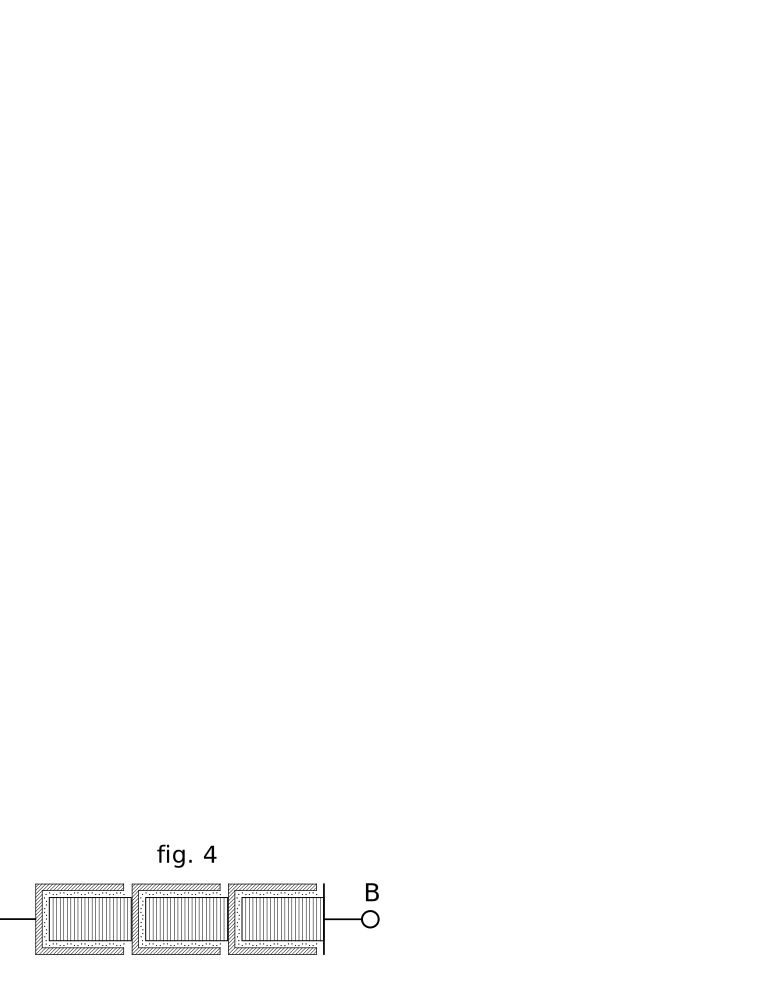
\includegraphics[width=0.40\textwidth]{gesamttex/edit_VIII,3/images/LH_35_09_16_002-003_d4.pdf}}%
  \vspace{0.4em}
  \centerline{\lbrack\textit{Fig.~4}\rbrack}%
  \label{LH_35_09_16_003r_Fig.4}%
 \newpage
\pstart
\noindent ut in \textit{10.11.}\edlabel{KZeitz94}
%
Fila\protect\index{Sachverzeichnis}{filum} autem
quae
nobis visibilia\protect\index{Sachverzeichnis}{filum visibile}
\edtext{sunt ex}{%
\lemma{sunt}\Bfootnote{%
\hspace{-0,5mm}\textbar~forte \mbox{\textit{gestr.}}~\textbar\ ex%
~\textit{L}}}
%
multis millibus filamentorum\protect\index{Sachverzeichnis}{filamentum}
qualia depinximus constare credibile est,
ut videmus certe fila araneae\protect\index{Sachverzeichnis}{filum araneae}\protect\index{Sachverzeichnis}{aranea}
aut bombycis\protect\index{Sachverzeichnis}{filum bombycis}\protect\index{Sachverzeichnis}{bombyx}
semper adhuc in alia dividi posse,
et folia talci\protect\index{Sachverzeichnis}{folium talci}\protect\index{Sachverzeichnis}{talcum}
in alia folia posse resolvi donec visum\protect\index{Sachverzeichnis}{visus}
\edtext{fugiant.
Unde non est mirum tantam esse corporum quorundam tenacitatem.\protect\index{Sachverzeichnis}{tenacitas}
Nam insertionibus illis continuis\protect\index{Sachverzeichnis}{insertio continua}
prominentiae\protect\index{Sachverzeichnis}{prominentia} corporis unius in sinum\protect\index{Sachverzeichnis}{sinus} alterius,
cujus prominentia\protect\index{Sachverzeichnis}{prominentia} rursus in sinum\protect\index{Sachverzeichnis}{sinus} tertii intrat,
atque ita porro;
idem praestatur quod in\protect\index{Sachverzeichnis}{figura}
\edtext{fig.~4}{%
\lemma{fig.~4}\Cfootnote{%
Das Diagramm \lbrack\textit{Fig.~4}\rbrack\ auf S.~\pageref{LH_35_09_16_003r_Fig.4}.}}
si emboli\protect\index{Sachverzeichnis}{embolus} in tubos\protect\index{Sachverzeichnis}{tubus} inserantur,
et embolis\protect\index{Sachverzeichnis}{embolus} novi rursus tubi\protect\index{Sachverzeichnis}{tubus} adhaereant.
Item contactu\protect\index{Sachverzeichnis}{contactus partium} viciniaque\protect\index{Sachverzeichnis}{vicinia partium} 
partium in\protect\index{Sachverzeichnis}{figura}
\edtext{fig.~3}{%
\lemma{fig.~3}\Cfootnote{%
Das Dia\-gramm \lbrack\textit{Fig.~3}\rbrack\ auf 
S.~\pageref{LH_35_09_16_002v_Fig.3}.}}
idem praestatur quod}{%
\lemma{fugiant.}\Bfootnote{%
\textit{(1)}~Haec ergo fragmina idem praestabunt, quod plures tubi posito
\textit{(2)}~Unde non \lbrack...\rbrack\ quorundam tenacitatem. % est mirum tantam esse corporum
\textit{(a)}~Quoni
\textit{(b)}~Idem enim 
\textit{(c)}~Nam insertionibus illis
\textit{(aa)}~sinu
\textit{(bb)}~prominentiarum in sinus praestatur, quod
\textit{(cc)}~continuis prominentiae \lbrack...\rbrack\ quod in fig.
\textit{(aaa)}~7
\textit{(bbb)}~4
\textit{(aaaa)}~tubis
\textit{(bbbb)}~embolis in tubos insertis, in
\textit{(aaaaa)}~qui
\textit{(bbbbb)}~quibus emb
\textit{(cccc)}~si emboli \lbrack...\rbrack\ tubi adhaereant
\textit{(aaaaa)}~, vel in fig.~8
\textit{(bbbbb)}~. Item contactu
\textit{(aaaaa-a)}~et vicinia
\textit{(bbbbb-b)}~viciniaque
\textit{(aaaaa-aa)}~horum corporum
\textit{(bbbbb-bb)}~co
\textit{(ccccc-cc)}~fragmentor
\textit{(ddddd-dd)}~partium in fig.
\textit{(aaaaa-aaa)}~6
\textit{(bbbbb-bbb)}~3 idem praestatur,
\textit{(aaaaa-aaaa)}~quod
\textit{(bbbbb-bbbb)}~quod%
~\textit{L}}}
%
pluribus tabulis politis\protect\index{Sachverzeichnis}{tabula polita}
sibi immistis ut in\protect\index{Sachverzeichnis}{figura}
\edtext{fig.~5.}{%
{\lemma{fig.}\Bfootnote{%
\textit{(1)}~8.
\textit{(2)}~5.%
~\textit{L}}}%
{\lemma{fig.~5}\Cfootnote{%
Das Diagramm \lbrack\textit{Fig.~5}\rbrack.}}}
Et sciendum\edlabel{LH_35_09_16_003r_tabulae-1}
\edtext{}{%
{\xxref{LH_35_09_16_003r_tabulae-1}{LH_35_09_16_003r_tabulae-2}}%
{\lemma{sciendum \lbrack...\rbrack\ divelli}\Cfootnote{%
Siehe N.~14\textsubscript{2}, S.~\refpassage{LH_37_03_069r_duaetabulae-1}{LH_37_03_069r_duaetabulae-2},
und N.~14\textsubscript{5}.}}}% % VERWEIS AUF "De firmitate corporum" UND "De duabus tabulis"  !  !  !  !  !
%
\edtext{est tabulas}{%
\lemma{est}\Bfootnote{\textbar~duas \textit{gestr.}~\textbar\ tabulas%
~\textit{L}}}
%
marmoreas\protect\index{Sachverzeichnis}{tabula marmorea}
\edtext{politas,\protect\index{Sachverzeichnis}{tabula polita}
licet eas tanquam perfecte}{%
\lemma{politas,}\Bfootnote{%
\textit{(1)}~quas velut perfecte
\textit{(2)}~licet eas tanquam perfecte%
~\textit{L}}}
%
rigidas\protect\index{Sachverzeichnis}{tabula perfecte rigida} concipiamus,
non tamen primo separationis momento\protect\index{Sachverzeichnis}{momentum separationis} a se invicem
\edtext{divelli.\edlabel{LH_35_09_16_003r_tabulae-2}
Nam in\protect\index{Sachverzeichnis}{figura}
\edtext{fig.~6}{%
\lemma{fig.~6}\Cfootnote{%
Das Diagramm \lbrack\textit{Fig.~6a}\rbrack\ auf S.~\pageref{LH_35_09_16_003r_Fig.6}.}}
sint}{%
\lemma{divelli.}\Bfootnote{%
\textit{(1)}~Sit enim in fig.~9
\textit{(2)}~Nam in fig.
\textit{(a)}~9
\textit{(b)}~6 sint%
~\textit{L}}}
%
tres tabulae marmoreae\protect\index{Sachverzeichnis}{tabula marmorea} politae\protect\index{Sachverzeichnis}{tabula polita} sibi
\edtext{applicatae,\protect\index{Sachverzeichnis}{tabulae sibi applicatae} \textit{1.2.3},
quarum}{%
\lemma{applicatae,}\Bfootnote{%
\textit{(1)}~qua
\textit{(2)}~\textit{1.2.3}, quarum%
~\textit{L}}}
%
\edtext{suprema \textit{1} sit}{%
\lemma{suprema}\Bfootnote{%
\textit{(1)}~si
\textit{(2)}~\textit{1} sit%
~\textit{L}}}
fixa in loco superiore,
media \textit{2} ei subsit,
%
et huic tertia \textit{3},
cui appensum pondus.\protect\index{Sachverzeichnis}{pondus appensum}
\edtext{Hoc pondus\protect\index{Sachverzeichnis}{pondus appensum}
tabulas primo tam parum a se invicem removebit,}{%
\lemma{Hoc}\Bfootnote{%
\hspace{-0,5mm}\textbar~pondus \textit{erg.}~%
\textbar\ tabulas
\textit{(1)}~\textlangle undiq\textrangle\
\textit{(2)}~non 
\textit{(3)}~potest
\textit{(4)}~primo tam \lbrack...\rbrack\ se invicem % parum a
\textit{(a)}~removere
\textit{(b)}~removebit,%
~\textit{L}}}
%
ut aeri circumfuso\protect\index{Sachverzeichnis}{aer circumfusus} nondum pateat
\edtext{introitus\protect\index{Sachverzeichnis}{introitus aeris}\lbrack,\rbrack\
itaque}{%
\lemma{introitus}\Bfootnote{%
\textit{(1)}~et
\textit{(2)}~itaque%
~\textit{L}}}
%
non ante sequetur divulsio\protect\index{Sachverzeichnis}{divulsio}
quam ubi intercapedo\protect\index{Sachverzeichnis}{intercapedo} sufficiens erit aeri transmittendo.
Idem ergo dicendum est\edtext{}{\lemma{\hspace{1,6mm}\lbrack\textit{Fig.~5}\rbrack}\killnumber\Cfootnote{% 
Das Diagramm hieß ursprünglich \textit{fig.~8}.}}%
\pend
 \vspace{1.5em}
 \centerline{\includegraphics[width=0.42\textwidth]{gesamttex/edit_VIII,3/images/LH_35_09_16_002-003_d5.pdf}}% 
  \vspace*{0.5em}
  \centerline{\lbrack\textit{Fig.~5}\rbrack}% 
  \label{LH_35_09_16_003r_Fig.5}%
  \newpage
  \pstart 
\begin{minipage}[t][1.9cm][b]{0.5\textwidth}
\hspace{-2mm}\includegraphics[width=0.82\textwidth]{gesamttex/edit_VIII,3/images/LH_35_09_16_002-003_d6a.pdf}
\end{minipage}
\hspace{12mm}
\begin{minipage}[t][2cm][t]{0.5\textwidth}
\includegraphics[width=0.47\textwidth]{gesamttex/edit_VIII,3/images/LH_35_09_16_002-003_d6b.pdf}
\end{minipage}
\\
\\
\hspace*{25.5mm} [\textit{Fig.~6a}]\hspace*{52mm} [\textit{Fig.~6b, gestr.}] \label{LH_35_09_16_003r_Fig.6}
\pend
\vspace{2.0em}
%  \vspace*{0.0em}%					Diagramm Fig.~6a
%  \centerline{\hspace*{-64mm}\includegraphics[width=0.42\textwidth]{gesamttex/edit_VIII,3/images/LH_35_09_16_002-003_d6a.pdf}}%
%  \vspace*{0.5em}
%  \centerline{\hspace*{-64mm}\lbrack\textit{Fig.~6a}\rbrack}%
%  \label{LH_35_09_16_003r_Fig.6}%
%%  \vspace*{1.5em}%
%%
%  \vspace*{-8.0em}%					Diagramm Fig.~6b
%  \centerline{\hspace*{70mm}\includegraphics[width=0.22\textwidth]{gesamttex/edit_VIII,3/images/LH_35_09_16_002-003_d6b.pdf}}% \hspace*{42mm}
%  \vspace*{0.75em}
%  \centerline{\hspace*{70mm}\lbrack\textit{Fig.~6b, gestr.}\rbrack}% \hspace*{42mm}
%  \vspace*{4.0em}%
%
 \pstart
\noindent%
% % % % % %       A C H T U N G   G E T R I X T       ! ! ! ! ! 
%
\edtext{}{\lemma{\hspace{1,6mm}\lbrack\textit{Fig.~6a}\rbrack}\killnumber\Cfootnote{% 
Das Diagramm hieß ursprünglich \textit{fig.~9}.}}%
\setline{1}in\protect\index{Sachverzeichnis}{figura}
\edlabel{KZeitz85}\edtext{}{{\xxref{KZeitz85}{KZeitz86}}%
{%
\lemma{fig.}\Bfootnote{%
\textit{(1)}~6,
\textit{(2)}~3,%
~\textit{L}}}}%
fig.~3,\edlabel{KZeitz86}
%
et proinde filamenta\protect\index{Sachverzeichnis}{filamentum} tamdiu extendentur
donec
\edtext{tandem separatio partium\protect\index{Sachverzeichnis}{separatio partium}
ex quibus constant sufficiens fiat}{%
\lemma{tandem}\Bfootnote{%
\textit{(1)}~superet
\textit{(2)}~separatio partium \lbrack...\rbrack\ sufficiens fiat%
~\textit{L}}}
%
\edtext{ad fluidum illud}{%
\lemma{ad}\Bfootnote{%
\textit{(1)}~aerem
\textit{(2)}~fluidum illlud%
~\textit{L}}}
%
elasticum,\protect\index{Sachverzeichnis}{fluidum elasticum}
quod aere communi\protect\index{Sachverzeichnis}{aer communis} subtilius
\edtext{esse\lbrack,\rbrack\ crassitiem tamen suam habere duximus}{%
\lemma{esse}\Bfootnote{%
\hspace{-0,5mm}crassitiem \lbrack...\rbrack\ habere duximus % tamen suam
\textit{erg.~L}}}\lbrack,\rbrack\
%
transmittendum;
itaque eaedem leges\protect\index{Sachverzeichnis}{lex}
quae in aere communi,\protect\index{Sachverzeichnis}{aer communis}
\edtext{hic}{%
\lemma{hic}\Bfootnote{%
\textit{erg.~L}}}
%
locum habebunt.
% % % % % %       A C H T U N G   G E T R I X T       ! ! ! ! ! 
% \edtext{}{\lemma{\lbrack\textit{Fig.~4}\rbrack}\killnumber\Cfootnote{%
% Das Diagramm hieß ursprünglich \textit{fig.~7}.}}%
% \edtext{}{\lemma{\hspace{1,6mm}\lbrack\textit{Fig.~5}\rbrack}\killnumber\Cfootnote{%
% Das Diagramm hieß ursprünglich \textit{fig.~8}.}}%
%
\pend%
 %					Diagramm Fig.~5
  %
%% \newpage%
%%
%%
\pstart%
%
Etsi autem Tubus\protect\index{Sachverzeichnis}{tubus} unus in
\edtext{fig.~4}{%
{\lemma{fig.}\Bfootnote{%
\textit{(1)}~7
\textit{(2)}~4%
~\textit{L}}}%
{\lemma{fig.~4}\Cfootnote{%
Das Diagramm \lbrack\textit{Fig.~4}\rbrack\ auf 
S.~\pageref{LH_35_09_16_003r_Fig.4}.}}}
%
alio
\edtext{sit amplior,}{%
\lemma{sit}\Bfootnote{%
\textit{(1)}~latior
\textit{(2)}~amplior,%
~\textit{L}}}
%
vel in\protect\index{Sachverzeichnis}{figura}
\edtext{fig.~3}{%
{\lemma{fig.}\Bfootnote{%
\textit{(1)}~6
\textit{(2)}~3%
~\textit{L}}}%
{\lemma{fig.~3}\Cfootnote{%
Das Diagramm \lbrack\textit{Fig.~3}\rbrack\ auf 
S.~\pageref{LH_35_09_16_002v_Fig.3}.%
}}}
%
unum planum contactus\protect\index{Sachverzeichnis}{planum contactus}
ut \textit{1.2} alio ut \textit{12.13}
\edtext{majus,
tamen cum \textit{A} et \textit{B} in diversa trahuntur,
simul omnes partes distrahentur,}{%
\lemma{majus,}\Bfootnote{\hspace{-0,5mm}% 
\textbar~(\protect\vphantom)%
neque enim sinuositas\protect\index{Sachverzeichnis}{sinuositas} sua consideranda est,
sed planum ad lineam distrationis \textit{AB} perpendiculare%
\protect\vphantom() \textit{gestr.}~%
\textbar\ tamen
\textit{(1)}~distrahendo
\textit{(2)}~cum \textit{A} et \textit{B} in diversa
\textit{(a)}~dis
\textit{(b)}~trahuntur, simul omnes partes
\textbar~vel tubi \textit{gestr.}~%
\textbar\ distrahentur,%
~\textit{L}}}
%
omnesve emboli\protect\index{Sachverzeichnis}{embolus}
\edtext{extrahentur uniformi quaedam difformitate,\protect\index{Sachverzeichnis}{difformitas uniformis}
nam ubique ita moderanda est extractio illa simultanea\protect\index{Sachverzeichnis}{extractio simultanea}
ut spatia aeris inclusi\protect\index{Sachverzeichnis}{aer inclusus} proportionaliter augeantur,
seu ut uno in duplum spatium\protect\index{Sachverzeichnis}{spatium aeris} dilatato,
etiam alter fiat duplo rarior\lbrack;\rbrack\
et proinde ruptura\protect\index{Sachverzeichnis}{ruptura} continget
caeteris paribus in loco maxime sinuoso,\protect\index{Sachverzeichnis}{locus maxime sinuosus}
ubi maxima est distractio,\protect\index{Sachverzeichnis}{distractio maxima} ibi enim}{%
\lemma{extrahentur}\Bfootnote{%
\textit{(1)}~magis tamen illi quorum tubi sunt angustiores % //((magi)) 
\textit{(2)}~uniformi quaedam difformitate,
\textbar~%
\textit{(1)}~extractione angustiam compensantem
\textit{(2)}~nam ubique \lbrack...\rbrack\ simultanea ut
\textit{(a)}~si unus aer unius
\textit{(b)}~spatia aeris \lbrack...\rbrack\ duplo rarior
\textit{erg.}~\textbar\ et proinde ruptura continget
\textit{(a)}~in tubo vel breviore vel angustiore, aut
\textit{(b)}~in contactu illo, ubi
\textit{(c)}~caeteris paribus \lbrack...\rbrack\ ibi enim%
~\textit{L}}}
%
primum sufficiens\protect\index{Sachverzeichnis}{aditus sufficiens}
\edtext{fluido externo\protect\index{Sachverzeichnis}{fluidum externum} aditus datur.}{%
\lemma{fluido}\Bfootnote{%
\textit{(1)}~via datur
\textit{(2)}~externo aditus datur.%
~\textit{L}}}
%
Licet autem plures tubi conjuncti\protect\index{Sachverzeichnis}{tubus conjunctus}
\edtext{intelligantur,
ut in fig.~4,% 
% \edtext{}{%\lemma{fig.~4}\Cfootnote{% Das Diagramm \lbrack\textit{Fig.~4}\rbrack\ auf S.~\pageref{LH_35_09_16_003r_Fig.4}.}}%
}{%
\lemma{intelligantur,}\Bfootnote{%
\textit{(1)}~ut in
\textit{(2)}~ut in fig.
\textit{(a)}~7,
\textit{(b)}~4,%
~\textit{L}}}
%
iique capacitate\protect\index{Sachverzeichnis}{capacitas tubi} inaequales,
tamen in singulis verum
\pend
\newpage
\pstart
\noindent
\edlabel{KZeitz95}\edtext{}{{\xxref{KZeitz95}{KZeitz96}}%
{%
\lemma{erit,}\Bfootnote{%
\textit{(1)}~\textbar~embolorum \textit{erg.}~\textbar\ extractiones, seu totius filamenti
\textit{(a)}~ex iis compositi
\textit{(b)}~ex his tubis vel partibus sinuosis compositi
\textit{(2)}~per
\textit{(a)}~ostens
\textit{(b)}~ostensa ad fig.
\textit{(aa)}~\textlangle5\textrangle\
\textit{(bb)}~2
\textit{(aaa)}~extensiones
\textit{(bbb)}~(\protect\vphantom)ac proinde et in toto
\textit{(aaaa)}~ex iis
\textit{(bbbb)}~filamento ex iis composito\protect\vphantom(),
\textit{(aaaaa)}~extensiones, seu
\textit{(bbbbb)}~quod asserimus, \lbrack...\rbrack\ vel distractiones
\textit{(aaaaa-a)}~partium vicinarum
\textit{(bbbbb-b)}~vicinitatum,%
~\textit{L}}}}%
erit,
per ostensa ad\protect\index{Sachverzeichnis}{figura}
\edtext{fig.~2}{%
\lemma{fig.~2}\Cfootnote{%
Das Diagramm \lbrack\textit{Fig.~2}\rbrack\ auf 
S.~\pageref{LH_35_09_16_002v_Fig.2}.}}
(\protect\vphantom)%
ac proinde et in toto filamento\protect\index{Sachverzeichnis}{filamentum} ex iis composito%
\protect\vphantom(),
\edtext{quod asseruimus,}{%
\lemma{quod asseruimus}\Cfootnote{%
Vgl. S.~\refpassage{LH_35_09_16_002v_asseruimus-1}{LH_35_09_16_002v_asseruimus-2}.}}
nempe extractiones embolorum\protect\index{Sachverzeichnis}{extractio emboli}
seu prominentiarum\protect\index{Sachverzeichnis}{prominentia}
ex tubis\protect\index{Sachverzeichnis}{tubus} vel sinubus,\protect\index{Sachverzeichnis}{sinus}
vel distractiones\protect\index{Sachverzeichnis}{distractio} vicinitatum,\protect\index{Sachverzeichnis}{vicinitas}
adeoque totius filamenti extensiones,\protect\index{Sachverzeichnis}{extensio filamenti}\edlabel{KZeitz96}
%
fore
\edtext{viribus extendentibus\protect\index{Sachverzeichnis}{vis tendens}
proportionales,\protect\index{Sachverzeichnis}{extensio proportionalis}}{%
\lemma{viribus}\Bfootnote{%
\textit{(1)}~proportionales
\textit{(2)}~extendentibus proportionales,%
~\textit{L}}}
%
quia si proportionalibus proportionalia addantur,
tota proportionalia sunt.
\pend%
%\newpage
\pstart
Quod ut appareat distinctus,
sint in\protect\index{Sachverzeichnis}{figura}
\edtext{fig.~7}{%
\lemma{fig.~7}\Cfootnote{%
Das Diagramm \lbrack\textit{Fig.~7d}\rbrack\ auf S.~\pageref{LH_35_09_16_003r_Fig.7}.}}
%
tria corpuscula\protect\index{Sachverzeichnis}{corpusculum distractum}
hoc ordine\protect\index{Sachverzeichnis}{ordo} sibi apposita:
\textit{ab}\edtext{\lbrack\textit{m}\rbrack,}{%
\lemma{\textit{m}}\Bfootnote{%
\textit{erg. Hrsg.}}}
%
\textit{cd}\edtext{\lbrack\textit{n}\rbrack,}{%
\lemma{\textit{n}}\Bfootnote{%
\textit{erg. Hrsg.}}}
%
\textit{efg}
et prope sibi admota in situ primo,
at in situ\protect\index{Sachverzeichnis}{situs}
\edtext{secundo per appensum pondus \textit{K}\protect\index{Sachverzeichnis}{pondus appensum}
distracta,\protect\index{Sachverzeichnis}{corpusculum distractum} ita quidem,}{%
\lemma{secundo}\Bfootnote{%
\textit{(1)}~ita
\textit{(2)}~per appensum pondus \textit{K}
\textit{(a)}~ita
\textit{(b)}~distracta, ita quidem,%
~\textit{L}}}
%
ut aer comprehensus\protect\index{Sachverzeichnis}{aer comprehensus} antea in spatio
\textit{\footnotesize{1}\normalsize{b}\footnotesize{1}\normalsize{c}\footnotesize{1}\normalsize{m}}
nunc occupet spatium duplum
\textit{\footnotesize{2}\normalsize{b}\footnotesize{2}\normalsize{c}\footnotesize{2}\normalsize{m}},
itaque similiter spatium\protect\index{Sachverzeichnis}{spatium aeris}
\textit{\footnotesize{2}\normalsize{d}\footnotesize{2}\normalsize{e}\footnotesize{2}\normalsize{h}\footnotesize{2}\normalsize{g}\footnotesize{2}\normalsize{n}}
debet esse duplum spatii
\textit{\footnotesize{1}\normalsize{d}\footnotesize{1}\normalsize{e}\footnotesize{1}\normalsize{h}\footnotesize{1}\normalsize{g}\footnotesize{1}\normalsize{n}},
\edtext{seu rectangulum\protect\index{Sachverzeichnis}{rectangulum}}{%
\lemma{seu}\Bfootnote{%
\textit{(1)}~parallelogrammum\protect\index{Sachverzeichnis}{parallelogrammum}
\textit{(2)}~rectangulum%
~\textit{L}}}
%
quod
\edtext{accessit\lbrack,\rbrack\ nempe
\textit{\footnotesize{2}\normalsize{d}\footnotesize{2}\normalsize{e}\footnotesize{2}\normalsize{g}\footnotesize{2}\normalsize{n}}}{%
\lemma{accessit}\Bfootnote{%
\textit{(1)}~spatio ut \textit{\footnotesize{2}\normalsize{d}\footnotesize{2}\normalsize{e}}
\textit{(2)}~nempe \textit{\footnotesize{2}\normalsize{d}\footnotesize{2}\normalsize{e}\footnotesize{2}\normalsize{g}\footnotesize{2}\normalsize{n}}%
~\textit{L}}}\lbrack,\rbrack\
%
ipsi
\textit{\footnotesize{1}\normalsize{d}\footnotesize{1}\normalsize{e}\footnotesize{1}\normalsize{h}\footnotesize{1}\normalsize{g}\footnotesize{1}\normalsize{n}}
aequale.
Hinc si in tertio situ\protect\index{Sachverzeichnis}{situs} pondus appendatur \textit{L},
duplum ponderis \textit{K},\protect\index{Sachverzeichnis}{pondus appensum}
adhuc semel tantundem spatii\protect\index{Sachverzeichnis}{spatium aeris}
\edtext{accedet, aerisque dilatatio\protect\index{Sachverzeichnis}{dilatatio aeris} duplicabitur,}{%
\lemma{accedet,}\Bfootnote{%
\textit{(1)}~nempe quantum spatium aeris
\textit{(2)}~aerisque dilatatio duplicabitur,%
~\textit{L}}}
%
eritque spatium % //\footnotesize{3}\normalsize{b}\footnotesize{3}\normalsize{c}\footnotesize{??}\normalsize{??}}//
\textit{\footnotesize{3}\normalsize{b}\footnotesize{3}\normalsize{c}\footnotesize{3}\normalsize{m}}
triplum ipsius
\textit{\footnotesize{1}\normalsize{b}\footnotesize{1}\normalsize{c}\footnotesize{1}\normalsize{m}},
et
\textit{\footnotesize{3}\normalsize{d}\footnotesize{3}\normalsize{e}\footnotesize{3}\normalsize{h}\footnotesize{3}\normalsize{g}\footnotesize{3}\normalsize{n}}
triplum ipsius
\textit{\footnotesize{1}\normalsize{d}\footnotesize{1}\normalsize{e}\footnotesize{1}\normalsize{h}\footnotesize{1}\normalsize{g}\footnotesize{1}\normalsize{n}},
et ut in secundo situ
\edtext{ad spatium\protect\index{Sachverzeichnis}{spatium aeris}
\textit{\footnotesize{2}\normalsize{e}\footnotesize{2}\normalsize{h}\footnotesize{2}\normalsize{g}}
accessit aequale ipsi}{%
\lemma{ad}\Bfootnote{%
\textit{(1)}~\textit{\footnotesize{2}\normalsize{e}\footnotesize{2}\normalsize{f}\footnotesize{2}\normalsize{h}\footnotesize{2}\normalsize{g}}
\textit{(2)}~spatium \textit{\footnotesize{2}\normalsize{e}\footnotesize{2}\normalsize{h}\footnotesize{2}\normalsize{g}}
\textit{(a)}~aequale ipsi
\textit{(b)}~accessit aequale ipsi%
~\textit{L}}}
%
rectangulum\protect\index{Sachverzeichnis}{rectangulum}
\textit{\footnotesize{2}\normalsize{d}\footnotesize{2}\normalsize{e}\footnotesize{2}\normalsize{g}\footnotesize{2}\normalsize{n}},
ita in situ\protect\index{Sachverzeichnis}{situs} tertio rursus accedit tale rectangulum,
nam rectangulum\protect\index{Sachverzeichnis}{rectangulum}
\textit{\footnotesize{3}\normalsize{d}\footnotesize{3}\normalsize{e}\footnotesize{3}\normalsize{g}\footnotesize{3}\normalsize{n}}
est ipsius
\textit{\footnotesize{2}\normalsize{d}\footnotesize{2}\normalsize{e}\footnotesize{2}\normalsize{g}\footnotesize{2}\normalsize{n}}
duplum.
Unde
\edtext{patet sinuositatis\protect\index{Sachverzeichnis}{sinuositas}
ipsius spatii\protect\index{Sachverzeichnis}{spatium aeris} \textit{ehg} non haberi rationem,
sed tantum rectangulorum\protect\index{Sachverzeichnis}{rectangulum} ei aequalium,}{%
\lemma{patet}\Bfootnote{%
\textit{(1)}~non sinuositatem
\textit{(2)}~sinuositatis ipsius spatii \textit{ehg} non
\textit{(a)}~habere
\textit{(b)}~haberi rationem, sed tantum
\textit{(aa)}~rectanguli
\textit{(bb)}~rectangulorum ei
\textit{(aaa)}~aequalis,
\textit{(bbb)}~aequalium,%
~\textit{L}}}
%
sive horum
\edtext{altitudinum, nempe}{%
\lemma{altitudinum,}\Bfootnote{%
\textit{(1)}~nam
\textit{(2)}~nempe%
~\textit{L}}}
%
bases \textit{dn}, \textit{eg} semper manent,
altitudines variantur\lbrack:\rbrack\
\edtext{nam posterior}{%
\lemma{nam}\Bfootnote{%
\textit{(1)}~accessio secunda
\textit{(2)}~posterior%
~\textit{L}}}
%
\textit{\footnotesize{3}\normalsize{d}\footnotesize{3}\normalsize{e}}
est
\edtext{dupla ipsius
\textit{\footnotesize{2}\normalsize{d}\footnotesize{2}\normalsize{e}},}{%
\lemma{dupla}\Bfootnote{%
\textit{(1)}~accessionis prioris
\textit{(2)}~ipsius \textit{\footnotesize{2}\normalsize{d}\footnotesize{2}\normalsize{e}},%
~\textit{L}}}
%
et
\textit{\footnotesize{3}\normalsize{b}\footnotesize{3}\normalsize{c}}
tripla ipsius
\textit{\footnotesize{1}\normalsize{b}\footnotesize{1}\normalsize{c}}\lbrack;\rbrack\
et omnes computando
\edtext{altitudines, ut est}{%
\lemma{altitudines,}\Bfootnote{%
\textit{(1)}~erit
\textit{(2)}~ut est%
~\textit{L}}}
%
pondus \textit{K} ad pondus \textit{L},
ita est extensio facta a pondere \textit{K},
seu excessus\protect\index{Sachverzeichnis}{excessus} ipsius
\textit{\footnotesize{2}\normalsize{a}\footnotesize{2}\normalsize{f}}
super
\textit{\footnotesize{1}\normalsize{a}\footnotesize{1}\normalsize{f}},
ad extensionem\protect\index{Sachverzeichnis}{extensio proportionalis}
factam a pondere \textit{L},\protect\index{Sachverzeichnis}{pondus appensum}
seu ad excessum\protect\index{Sachverzeichnis}{excessus} ipsius
\textit{\footnotesize{3}\normalsize{a}\footnotesize{3}\normalsize{f}}
super
\textit{\footnotesize{1}\normalsize{a}\footnotesize{1}\normalsize{f}}.
Quod demonstrandum erat.
% \pend%
% \newpage%
% \pstart%
Manifestum est enim
eandem ratiocinatio- \makebox[1.0\textwidth][s]{nem\protect\index{Sachverzeichnis}{ratiocinatio} manere utcunque % //continu??//
multiplicatae sint partes componentes,\protect\index{Sachverzeichnis}{pars componens}
aut continuetur extensio,\protect\index{Sachverzeichnis}{extensio filamenti}}
\pend
\newpage
\pstart
\noindent
donec
\edtext{scilicet alicubi tantum fiat intervallum\protect\index{Sachverzeichnis}{intervallum} ut}{%
\lemma{scilicet}\Bfootnote{%
\textit{(1)}~tantum fiat intervallum ut alicubi
\textit{(2)}~alicubi tantum fiat intervallum ut%
~\textit{L}}}
%
fluido externo\protect\index{Sachverzeichnis}{fluidum externum}
detur aditus,\protect\index{Sachverzeichnis}{aditus sufficiens}
ubi nimirum ruptura\protect\index{Sachverzeichnis}{ruptura} continget.
Et quod de extensionibus,\protect\index{Sachverzeichnis}{extensio proportionalis}
idem eadem ratione de compressionibus\protect\index{Sachverzeichnis}{compressio} dicendum esse.%
\edlabel{LH_35_09_16_002v_Festigkeitsmodell_redg-2}
\pend
\vspace{3em}
\pstart\noindent
\begin{minipage}[t]{0.4\textwidth}
\includegraphics[width=1\textwidth]{gesamttex/edit_VIII,3/images/LH_35_09_16_002-003_d7a.pdf}
\end{minipage}
\hspace*{4mm}
\begin{minipage}[t]{0.26\textwidth}
\includegraphics[width=0.7\textwidth]{gesamttex/edit_VIII,3/images/LH_35_09_16_002-003_d7b.pdf}
\end{minipage}
\hspace*{-6mm}
\begin{minipage}[t]{0.33\textwidth}
\includegraphics[width=1\textwidth]{gesamttex/edit_VIII,3/images/LH_35_09_16_002-003_d7c.pdf}
\end{minipage}
\\
\\
\vspace{1em}
\setline{1}\hspace*{12mm} [\textit{Fig.~7a, gestr.}]\hspace*{21mm} [\textit{Fig.~7b, gestr.}]\hspace*{16mm} [\textit{Fig.~7c, gestr.}]
\vspace{1.5em}
\pend

%  \vspace*{3.0em}%					Diagramm Fig.~7a
%  \centerline{\hspace*{-85mm}\includegraphics[width=0.36\textwidth]{gesamttex/edit_VIII,3/images/LH_35_09_16_002-003_d7a.pdf}}% \hspace*{-64mm}
%  \vspace*{0.0em}
%  \centerline{\hspace*{-85mm}\lbrack\textit{Fig.~7a, gestr.}\rbrack}% \hspace*{-64mm}
%%
%%
%  \vspace*{1.0em}%					Diagramm Fig.~7b
%  \centerline{\includegraphics[width=0.16\textwidth]{gesamttex/edit_VIII,3/images/LH_35_09_16_002-003_d7b.pdf}}% \hspace*{-95mm}
%  \vspace*{0.0em}
%  \centerline{\lbrack\textit{Fig.~7b, gestr.}\rbrack}% \hspace*{-95mm}
%%
%%
%% \newpage%
%%
%%
%  \vspace*{-13.0em}%					Diagramm Fig.~7c
%  \centerline{\hspace*{90mm}\includegraphics[width=0.30\textwidth]{gesamttex/edit_VIII,3/images/LH_35_09_16_002-003_d7c.pdf}}% 
%  \vspace*{-1.5em}
%  \centerline{\hspace*{90mm}\lbrack\textit{Fig.~7c, gestr.}\rbrack}% 
%%
%%
%% \newpage%
%%
%
  \vspace{3em}%					Diagramm Fig.~7d
  \centerline{\includegraphics[width=0.92\textwidth]{gesamttex/edit_VIII,3/images/LH_35_09_16_002-003_d7d.pdf}}% \hspace*{-64mm}
  \vspace{0.5em}
  \centerline{\lbrack\textit{Fig.~7d}\rbrack}% \hspace*{-64mm}
  \label{LH_35_09_16_003r_Fig.7}%
  \count\Bfootins=1200
\count\Afootins=1200
\count\Cfootins=1200
%
%
% ENDE DES STÜCKES auf Blatt 3r